\documentclass{standalone}

\usepackage[usenames,dvipsnames]{xcolor}
\usepackage{tikz}
\usepackage{pgfplots}
\usepackage{graphicx}
\usepackage{comment}

\pgfplotsset{compat=newest}

\definecolor{IBM1}{HTML}{648fff}
\definecolor{IBM2}{HTML}{785ef0}
\definecolor{IBM3}{HTML}{dc267f}
\definecolor{IBM4}{HTML}{fe6100}
\definecolor{IBM5}{HTML}{ffb000}
\definecolor{IBM6}{RGB}{051,117,056}

\definecolor{Okabe1}{RGB}{000,158,115}
\definecolor{Okabe2}{RGB}{000,114,178}
\definecolor{Okabe3}{RGB}{086,180,233}
\definecolor{Okabe4}{RGB}{230,159,000}
\definecolor{Okabe5}{RGB}{213,094,000}
\definecolor{Okabe6}{RGB}{204,121,167}

\begin{document}
		\begin{tikzpicture}
		\begin{axis}[
			enlargelimits=false,
			title={$a.$},
			title style={yshift=-2ex, xshift=-33ex},
			tick pos=left, %
			tick align=outside, %
			axis line style={opacity=0}, %
			after end axis/.code={
				\draw ({rel axis cs:0,0}
				-|{axis cs:0,0}) % xmin (line starts here)
				-- ({rel axis cs:0,0}
				-|{axis cs:70,0}); % xmax (line stops here)
				\draw ({rel axis cs:0,0}
				|-{axis cs:0,0}) % ymin (line starts here)
				-- ({rel axis cs:0,0}
				|-{axis cs:0,2}); % ymax (line stops here)
			},
			grid=none,
			xlabel={$\theta$~(degrees)},
			ylabel={$F_c/F_c^0$},
			xmin=-3.5, xmax=70,
			ymin=0, ymax=2,
			legend style={
				at={(1,1)}, anchor=north east},
			scatter/classes={
				b={mark=triangle*, mark size=4pt,color = Okabe2, fill=Okabe2!80,opacity=0.7},
				c={mark=square*, mark size=3.5pt,color = Okabe3, fill=Okabe3!80,opacity=0.7},
				d={mark=diamond*, mark size=4pt,color = Okabe4, fill=Okabe4!80,opacity=0.7},
				e={mark=pentagon*, mark size=4pt,color = Okabe5, fill=Okabe5!80,opacity=0.7}
			}
			]
			
			\addplot[domain=0:1, color=Okabe1, dashed] coordinates{(20,0) (20,2)};
			\addplot[domain=0:1, color=Okabe6, dashed] coordinates{(32.36,0) (32.36,2)};
			\addlegendentry[scale=0.8]{$\theta_{dd} = 20^\circ$}
			\addlegendentry[scale=0.8]{$\theta_{id} \approx 32.4^\circ$}
			
			\addplot[scatter,only marks,% 
			scatter src=explicit symbolic, % Needed for scatter class styling
			error bars/.cd,
			x dir=both, x explicit,
			y dir=both, y explicit
			] 
			table[y error index=2, meta=label] {
				x y yerr label
				
				0	1.250945073	0.089061029	b
				11.28700002	1.370442095	0.053587298	b
				22.976	1.099136502	0.047159475	b
				35.29399999	1.03960685	0.020775689	b
				47.26899999	1.116592166	0.026631826	b
				
				0	1.490933931	0.027451553	c
				11.28700002	1.409452057	0.022340863	c
				22.976	1.155018504	0.032445517	c
				35.29399999	0.980939369	0.027606744	c
				47.26899999	1.117321696	0.008894032	c
				
				0	1.786367073	0.061291136	d
				11.28700002	1.425713945	0.052060591	d
				22.976	1.117003356	0.035343741	d
				35.29399999	0.946969797	0.006950432	d
				47.26899999	1.097491743	0.041226406	d
				
				0	1.906182436	0.046337096	e
				11.28700002	1.534427186	0.044370018	e
				22.976	1.123697347	0.069039558	e
				35.29399999	0.949370615	0.035422	e
				47.26899999	1.132774469	0.02851534	e
				
				
				
				
				
			};
			
			\addplot[domain=0:1, color=black, dashed] coordinates{(-3,1) (70,1)};

			\addlegendentry[scale=0.8]{$r_d=$~4 mm}
			\addlegendentry[scale=0.8]{$r_d=$~6 mm}
			\addlegendentry[scale=0.8]{$r_d=$~8 mm}
			\addlegendentry[scale=0.8]{$r_d=$~10 mm}
			
			
			
			\node[anchor=south] at (50, 0.05) {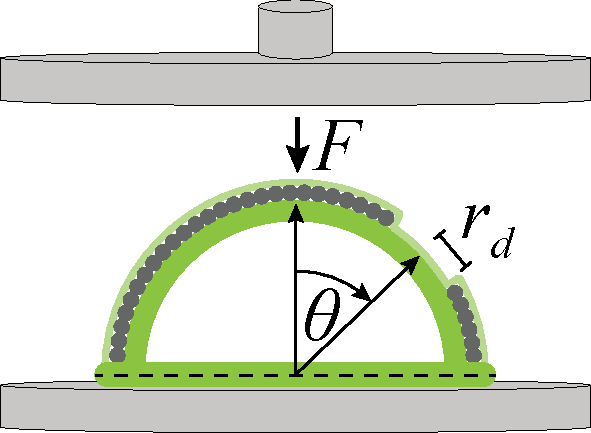
\includegraphics[height=1.75cm]{DefectAngleDiagram}};
		\end{axis}
		
	\end{tikzpicture}
	\vspace{1cm}
\end{document}